\documentclass[]{beamer}
% Class options include: notes, notesonly, handout, trans,
%                        hidesubsections, shadesubsections,
%                        inrow, blue, red, grey, brown

% Theme for beamer presentation.
\usepackage{beamerthemesplit} 



% Other themes include: beamerthemebars, beamerthemelined, 
%                       beamerthemetree, beamerthemetreebars  

\title{PHY115}    % Enter your title between curly braces
\author{Anabela R. Turlione}                 % Enter your name between curly braces
\institute{Digipen}      % Enter your institute name between curly braces
\date{Spring 2022}                    % Enter the date or \today between curly braces


\begin{document}

% Creates title page of slide show using above information
\begin{frame}
  \titlepage
\end{frame}
%\note{Talk for 30 minutes} % Add notes to yourself that will be displayed when
                           % typeset with the notes or notesonly class options

\section[]{}

% Creates table of contents slide incorporating
% all \section and \subsection commands
\begin{frame}
  \tableofcontents
\end{frame}

%%%%%%%%%%%%%%%%%%%%%%%%%%%%%%%%%%%%%%%%%%%%%%%%%%%%%%%%%%%%%%%%%%%
\section{Light}
\subsection{Introduction}


%%%%%%%%%%%%%%%%%%%%%%%%%%%%%%%%%%%%%%%%%%%%%%%%%%%%%%%%%%%%%%%%%%%
\begin{frame}
  \frametitle{Introduction}
  
What is light?
\pause
\vspace{10mm}

Light is Electromagnetic radiation


  
    \end{frame}
  
  %%%%%%%%%%%%%%%%%%%%%%%%%%%%%%%%%%%%%%%%%%%%%%%%%%%%%%%%%%%%%%%%%%%

%%%%%%%%%%%%%%%%%%%%%%%%%%%%%%%%%%%%%%%%%%%%%%%%%%%%%%%%%%%%%%%%%%%
\begin{frame}
\frametitle{Introduction}


\begin{itemize}
 \item  Changing Magnetic Field $\rightarrow$ Changing Electric Field
\pause 

\item Changing Electric Field $\rightarrow$ Changing Magnetic Field
\end{itemize}

\vspace{3mm}


\textbf{Electromagnetic Wave}: Wave of Electric and Magnetic Field
\pause
\vspace{3mm}

Changing Electric Field $\rightarrow$ Changing Magnetic Field$\rightarrow$ Changing Electric Field 

\pause
\vspace{3mm}

The light is an electromagnetic wave that can propagate through space.

  \end{frame}

%%%%%%%%%%%%%%%%%%%%%%%%%%%%%%%%%%%%%%%%%%%%%%%%%%%%%%%%%%%%%%%%%%%


\begin{frame}
\frametitle{Introduction}

To describe an electromagnetic wave we have to know first:
\pause

\begin{itemize}
 \item what is an Electric Field? 
\pause 

\item what is a Magnetic Field? 
\end{itemize}


  \end{frame}
%%%%%%%%%%%%%%%%%%%%%%%%%%%%%%%%%%%%%%%%%%%%%%%%%%%%%%%%%%%%%%%%%%%
\subsection{Electric Field}

\begin{frame}
\frametitle{Electric Field}

Force between two point charged particles:
\vspace{3mm}

\pause

\begin{center}
  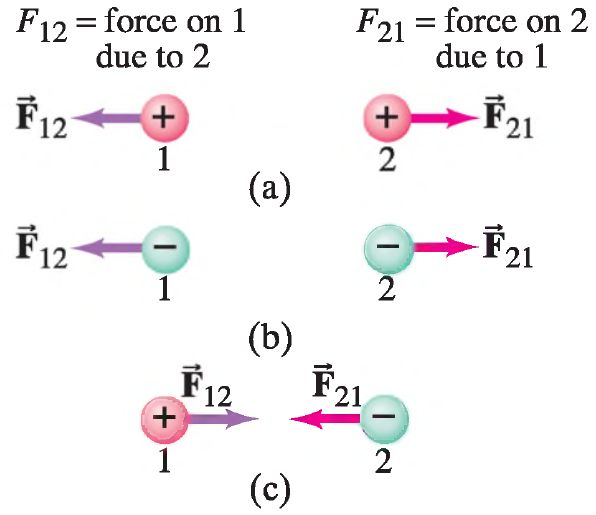
\includegraphics[height=1.7in]{images5/1.jpg}
\end{center}

%    \begin{columns}[c]
%    \column{2in}  % slides are 3in high by 5in wide

%     \begin{center}
%   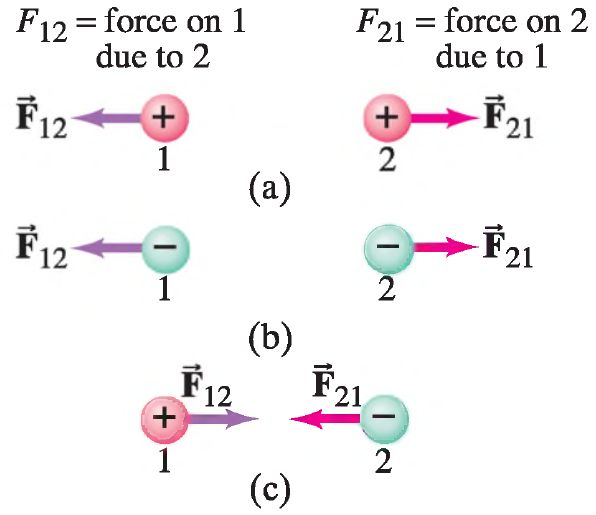
\includegraphics[height=1.7in]{images5/1.jpg}
% \end{center}



%    \column{2in}
% \pause

% \begin{equation}
% \vec{F_{12}}=\frac{1}{4\pi \epsilon_0}\frac{Q_1Q_2}{r_{12}^2}\hat{r}_{12}
% \end{equation}
% \pause


% Where $\epsilon_0$ is the permitivity of free space,
% \pause

% \begin{equation}
% \epsilon_0=8.85\times10^{-12} \frac{C^2}{Nm^2}
% \end{equation}



%   \end{columns}






  \end{frame}

%%%%%%%%%%%%%%%%%%%%%%%%%%%%%%%%%%%%%%%%%%%%%%%%%%%%%%%%%%%%%%%%%%%



% \begin{frame}
% \frametitle{Electric Field}

% 1C $\rightarrow$ one Coulomb:

% \vspace{3mm}
% \pause

% Amount of charge which, if placed on each of 2 point objects that are $1~m$ apart, result in a force of:


% \vspace{3mm}
% \pause

% \begin{equation}
% F=9\times 10^9 \frac{N\cdot m^2}{C^2}\frac{(1C)(1C)}{1~m^2}=9\times10^9~N
% \end{equation}

% \vspace{3mm}
% \pause

% Charge of one electron: $e=1.602\times 10^{-19}~C$

% \vspace{3mm}
% \pause

% Elementary charge $\rightarrow$ smalest charge found in nature
% \vspace{3mm}
% \pause

% charge $\propto n\cdot e$, $n$ integer, it is quantized.
%  \end{frame}

%%%%%%%%%%%%%%%%%%%%%%%%%%%%%%%%%%%%%%%%%%%%%%%%%%%%%%%%%%%%%%%%%%%




% \begin{frame}
% \frametitle{Electric Field}

% Electric field:

% \begin{equation}
% \vec{E}=\frac{\vec{F}}{q}
% \end{equation}

% \pause
% \vspace{3mm}

% $\vec{F}\rightarrow$ Force on a small positive test particle $q$.
% \pause
% \vspace{3mm}

% \begin{equation}
% [E]=\frac{N}{C}
% \end{equation}
% \pause
% \vspace{3mm}

% Then, the electric field generated by a charge $Q$ is:

% \begin{equation}
% E=\frac{1}{4\pi\epsilon_0}\frac{Q}{r^2}
% \end{equation}


%   \end{frame}

%%%%%%%%%%%%%%%%%%%%%%%%%%%%%%%%%%%%%%%%%%%%%%%%%%%%%%%%%%%%%%%%%%%







%%%%%%%%%%%%%%%%%%%%%%%%%%%%%%%%%%%%%%%%%%%%%%%%%%%%%%%%%%%%%%%%%%%
\subsection{Magnetic Field}

\begin{frame}
\frametitle{Magnetic Field}



Sources of Magnetic Fields: Ampere's Law

\begin{center}
  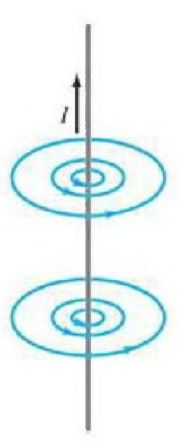
\includegraphics[height=1.5in]{images5/B.jpg}
\end{center}

\pause

The magnetic field generated by a straight wire is circular


  \end{frame}

%%%%%%%%%%%%%%%%%%%%%%%%%%%%%%%%%%%%%%%%%%%%%%%%%%%%%%%%%%%%%%%%%%%


% \begin{frame}
% \frametitle{Magnetic Field}

% The unit of the magnetic field is Tesla,

% \begin{equation}
% [B]=\frac{N}{A m}
% \end{equation}

% The constant $\mu_0$ is the \textbf{Vacuum Magnetic  Permeability}.

% \begin{equation}
% \mu_0=4\pi \times 10^{-7} \frac{T}{m A}
% \end{equation}



%   \end{frame}




%%%%%%%%%%%%%%%%%%%%%%%%%%%%%%%%%%%%%%%%%%%%%%%%%%%%%%%%%%%%%%%%%%%

% \begin{frame}
% \frametitle{Force due to a Magnetic Field}



% Force on a current  due to a magnetic Field:
% \vspace{3mm}

% \pause
% \begin{equation}
% \vec{F}=I\vec{\ell}\times \vec{B}
% \end{equation}
% \pause
% \vspace{3mm}

% Force on a point charge  due to a magnetic Field:
% \vspace{3mm}
% \pause

% \begin{equation}
% \vec{F}=q\vec{v}\times \vec{B}
% \end{equation}







%   \end{frame}



%%%%%%%%%%%%%%%%%%%%%%%%%%%%%%%%%%%%%%%%%%%%%%%%%%%%%%%%%%%%%%%%%%%




% \begin{frame}
% \frametitle{Force due to a Magnetic Field}



% Total force due to an electric and magnetic field:

% \vspace{3mm}
% \pause

% \begin{equation}
% \vec{F}=q(\vec{E}+\vec{v}\times \vec{B})\rightarrow Lorentz~Equation
% \end{equation}






%   \end{frame}


%%%%%%%%%%%%%%%%%%%%%%%%%%%%%%%%%%%%%%%%%%%%%%%%%%%%%%%%%%%%%%%%%%%

\begin{frame}

Example: Magnet
   \begin{columns}[c]
   \column{2in}  % slides are 3in high by 5in wide

  \begin{center}
  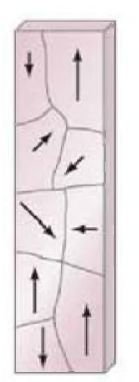
\includegraphics[height=1.5in]{images5/ferromagnetic.jpg}
\end{center}


   \column{2in}

\pause



In some materials called \textbf{Ferromagnetic}, the angular momentum of electrons are aligned so that they create a resultant macroscopic magnetic field.

\vspace{3mm}

\pause

Iron - Cobalt - Nickel

   \end{columns}









  \end{frame}



%%%%%%%%%%%%%%%%%%%%%%%%%%%%%%%%%%%%%%%%%%%%%%%%%%%%%%%%%%%%%%%%%%%
\subsection{Electromagnetic Radiation}

\begin{frame}

When the electric and magnetic fields are static, the are separate entities. But when they are changing,  we can not treat them separately 

\pause
\vspace{3mm}

$\rightarrow$ \textbf{Maxwell Equations}

\pause
\vspace{3mm}

A changing magnetic field generates a changing electric field that generates a changing magnetic field.

\pause
\vspace{3mm}

$\rightarrow$ \textbf{Wave traveling in the espace}

  \end{frame}





%%%%%%%%%%%%%%%%%%%%%%%%%%%%%%%%%%%%%%%%%%%%%%%%%%%%%%%%%%%%%%%%%%%



\begin{frame}


   \begin{columns}[c]
   \column{2in}  % slides are 3in high by 5in wide
  
  \begin{center}
  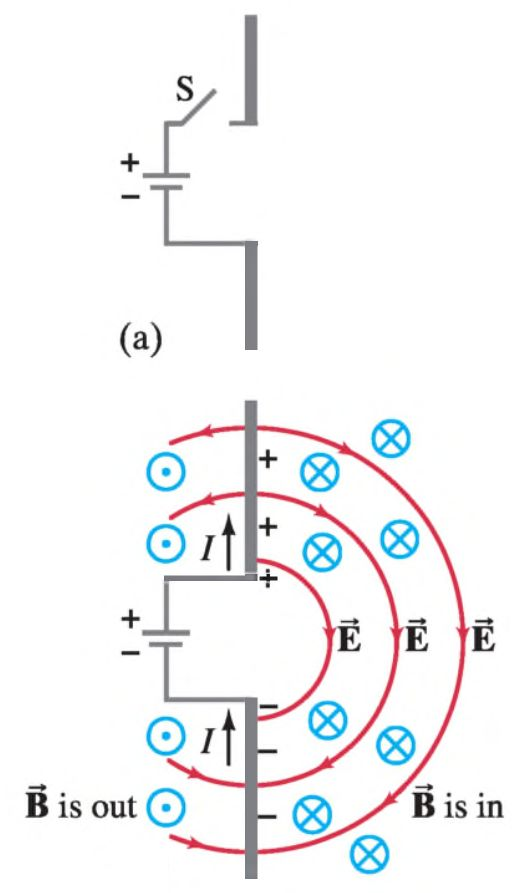
\includegraphics[height=2.3in]{images5/antenna1.jpg}
\end{center}


   \column{2.7in}


\begin{itemize}
\pause
\item We connect two rod to a battery $\rightarrow$ Electric Field 
\pause
\item  The charge is re-distributed $\rightarrow$  Magnetic field 

\end{itemize}

   \end{columns}


  \end{frame}


%%%%%%%%%%%%%%%%%%%%%%%%%%%%%%%%%%%%%%%%%%%%%%%%%%%%%%%%%%%%%%%%%%%



\begin{frame}


   \begin{columns}[c]
   \column{2in}  % slides are 3in high by 5in wide
  
  \begin{center}
  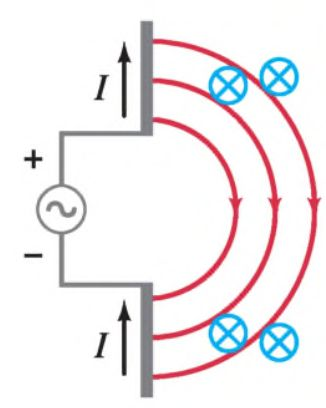
\includegraphics[height=1.7in]{images5/antenna2.jpg}
\end{center}


   \column{2.7in}


\begin{itemize}
\pause
\item sinusoidal voltage   $\rightarrow$ Alternating Current
\pause
\item $\rightarrow$ variable Electric and Magnetic Fields.
\end{itemize}

   \end{columns}


  \end{frame}


%%%%%%%%%%%%%%%%%%%%%%%%%%%%%%%%%%%%%%%%%%%%%%%%%%%%%%%%%%%%%%%%%%%






\begin{frame}


   \begin{columns}[c]
   \column{2in}  % slides are 3in high by 5in wide
  
  \begin{center}
  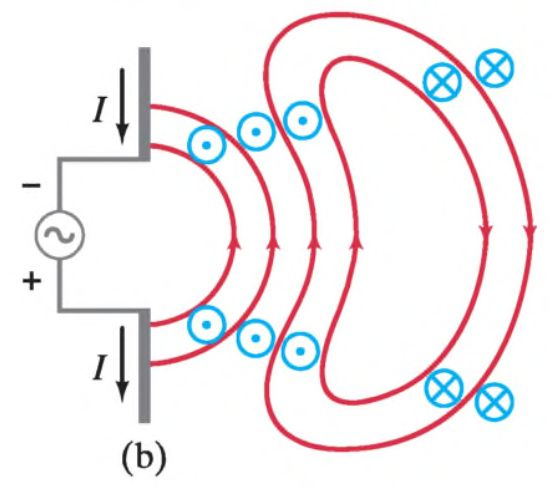
\includegraphics[height=1.7in]{images5/antenna3.jpg}
\end{center}


   \column{2.7in}


\begin{itemize}
\pause
\item Old Field lines fold back to connect to some of the new lines $\rightarrow$ closed loops
\pause
 \item The old field don't suddenly disappear
\pause
 \item changing EF $\rightarrow$ changing MF $\rightarrow$ changing EF ...$\rightarrow$ so on
\pause
 \item This combination of  changing EF and MF moving outward is self supporting, no longer depending on the antenna. 
\pause
 \item They are on their way to distant points.

\end{itemize}

   \end{columns}


  \end{frame}

%%%%%%%%%%%%%%%%%%%%%%%%%%%%%%%%%%%%%%%%%%%%%%%%%%%%%%%%%%%%%%%%%%%



\begin{frame}
\frametitle{Characteristics of Electromagnetic Waves}

\begin{itemize}

\item The field not far the antenna (\textit{Near Field}) is complicated.
\pause

\item The field far from the antenna (\textit{Far Field}) is quite flat $\rightarrow$ Plane Waves
\pause

\item The field also travels in other directions, the strength is greater in the direction perpendicular to the antenna.
\pause

\item The magnitude of $\vec{E}$ and $\vec{B}$ decreases with distance as $1/r$.
\pause

\item $\vec{E}\perp\vec{B}$, and they are $\perp$ to the direction of propagation.
\pause

\item  of $\vec{E}$ and $\vec{B}$ are in phase.

\end{itemize}

  \end{frame}


%%%%%%%%%%%%%%%%%%%%%%%%%%%%%%%%%%%%%%%%%%%%%%%%%%%%%%%%%%%%%%%%%%%



\begin{frame}
\frametitle{ Electromagnetic Waves}


 \begin{center}
  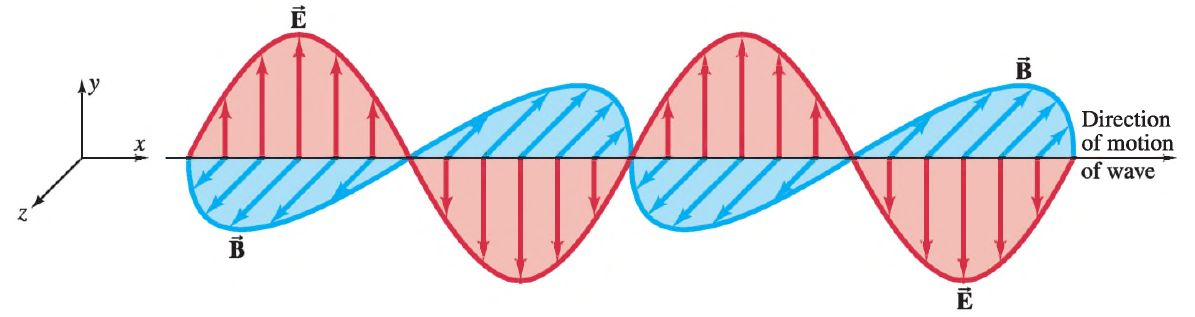
\includegraphics[height=0.6in]{images5/EMwave.jpg}
\end{center}


\begin{itemize}

 

\item Transverse wave
\pause 
\item Waves of field, not of matter
\pause
\item EM waves can propagate in empty space.

\pause
\vspace{3mm}
\pause

EM waves are produced by electric charges that are oscillating $\rightarrow$ are undergoing into acceleration in general.
\pause
\vspace{3mm}

\textbf{Accelerated electric charges give rise to electromagnetic waves}

\end{itemize}

  \end{frame}







%%%%%%%%%%%%%%%%%%%%%%%%%%%%%%%%%%%%%%%%%%%%%%%%%%%%%%%%%%%%%%%%%%%


% \begin{frame}


% We describe the waves as sinusoidal waves with wavelength $\lambda$ and frequency $f$:
% \pause
% \vspace{3mm}


% \begin{eqnarray}
% E=E_y&=&E_0sin(kx-\omega t)\\
% B=B_z&=&B_0sin(kx-\omega t)
% \end{eqnarray}
% \pause
% \vspace{3mm}

% where,
% \pause



% \begin{equation*}
% k=\frac{2\pi}{\lambda},\ \ \omega=2\pi f,\ \ f\lambda=\frac{\omega}{k}=v
% \end{equation*}


%   \end{frame}

%%%%%%%%%%%%%%%%%%%%%%%%%%%%%%%%%%%%%%%%%%%%%%%%%%%%%%%%%%%%%%%%%%%


% \begin{frame}

% \frametitle{Speed of light}



%    \begin{columns}[c]
%    \column{2in}  % slides are 3in high by 5in wide
  
%  \begin{center}
%   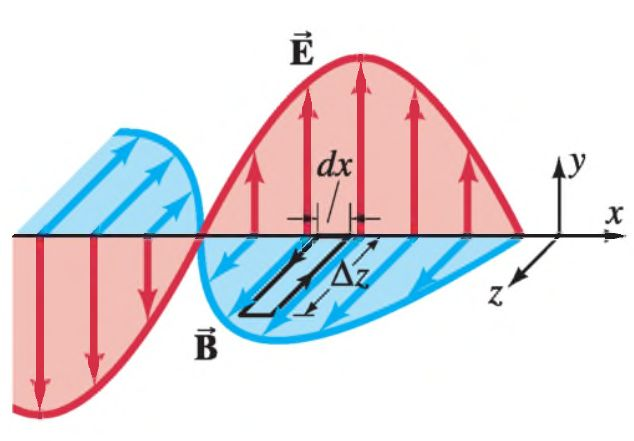
\includegraphics[height=1.4in]{images5/EMwave3.jpg}
% \end{center}


%    \column{2.5in}
% \pause

% The same with 

% \begin{equation*}
% \oint \vec{B}d\vec{\ell}=\mu_0\epsilon_0\frac{d\Phi_E}{dt}
% \end{equation*}
% \pause

% \begin{equation*}
% \rightarrow   \oint \vec{B}d\vec{\ell}=-(B+dB)\Delta y + B\delta y
% \end{equation*}
% \pause

% \begin{equation*}
% \rightarrow   \oint \vec{B}d\vec{\ell}=-dB\Delta y
% \end{equation*}
% \pause



%    \end{columns}




%   \end{frame}







%%%%%%%%%%%%%%%%%%%%%%%%%%%%%%%%%%%%%%%%%%%%%%%%%%%%%%%%%%%%%%%%%%%

% \begin{frame}

% \frametitle{Wave Equation}

% We can derive the speed of light without assuming sinusoidal waves...
% \pause
% The behaviour of light are decribed by Maxwel Equations.

% \pause

% With thouse equations we can prove that light propagates as a wave that travels at 

% $\sim 3\times 10^8 m / s$
%   \end{frame}




%%%%%%%%%%%%%%%%%%%%%%%%%%%%%%%%%%%%%%%%%%%%%%%%%%%%%%%%%%%%%%%%%%%




\begin{frame}

\frametitle{Measuring the speed of light}

Michelson's Experiment

  \begin{center}
  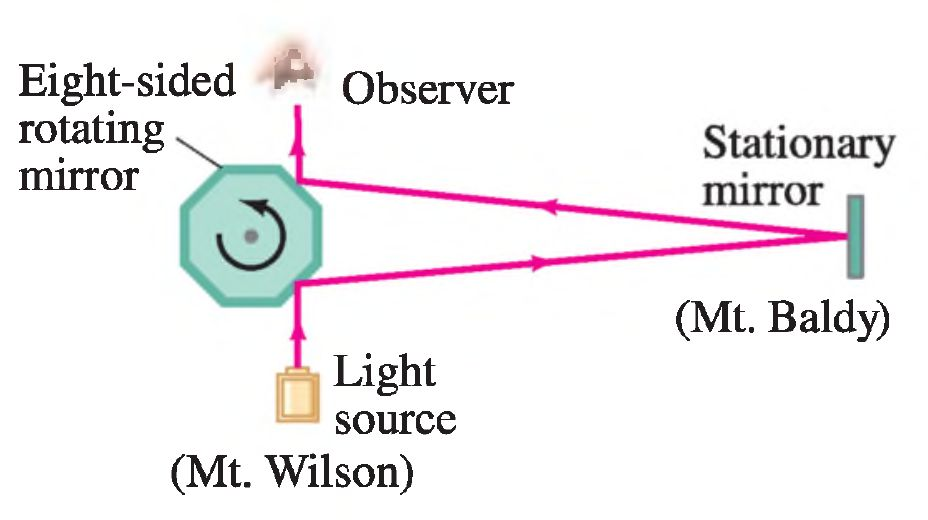
\includegraphics[height=2.0in]{images5/Michelson.jpg}
\end{center}




  \end{frame}

%%%%%%%%%%%%%%%%%%%%%%%%%%%%%%%%%%%%%%%%%%%%%%%%%%%%%%%%%%%%%%%%%%%


\begin{frame}

\frametitle{Electromagnetic spectrum}

The frequency of light is related with its speed thought the expression,

\begin{equation*}
c=f\lambda
\end{equation*}

  \begin{center}
  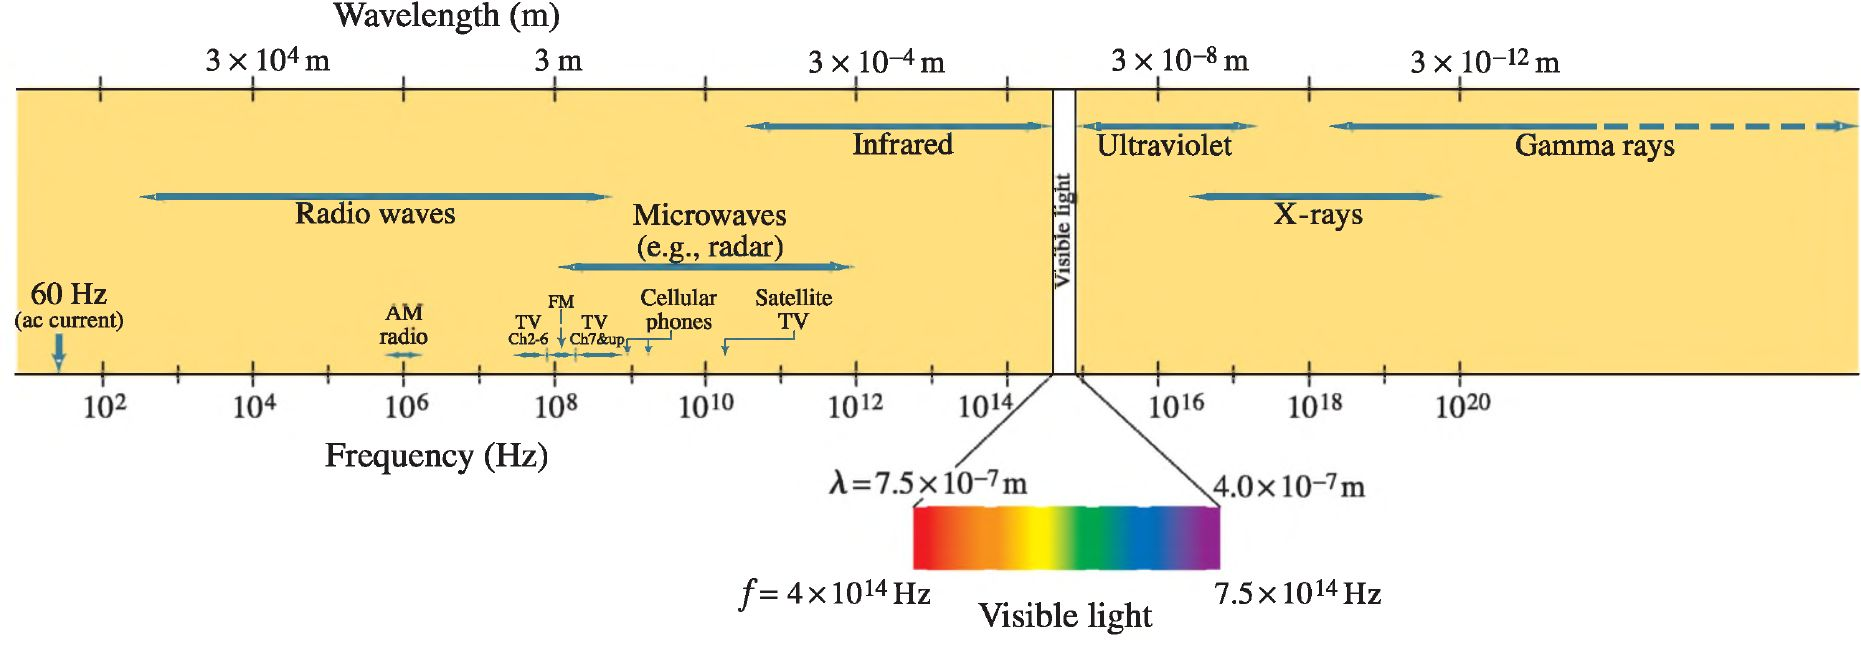
\includegraphics[height=1.5in]{images5/spectrum.jpg}
\end{center}



  \end{frame}


%%%%%%%%%%%%%%%%%%%%%%%%%%%%%%%%%%%%%%%%%%%%%%%%%%%%%%%%%%%%%%%%%%%


\begin{frame}

\frametitle{Electromagnetic spectrum}

The frequency of light is related with its speed thought the expression,

\begin{equation*}
c=f\lambda
\end{equation*}

  \begin{center}
  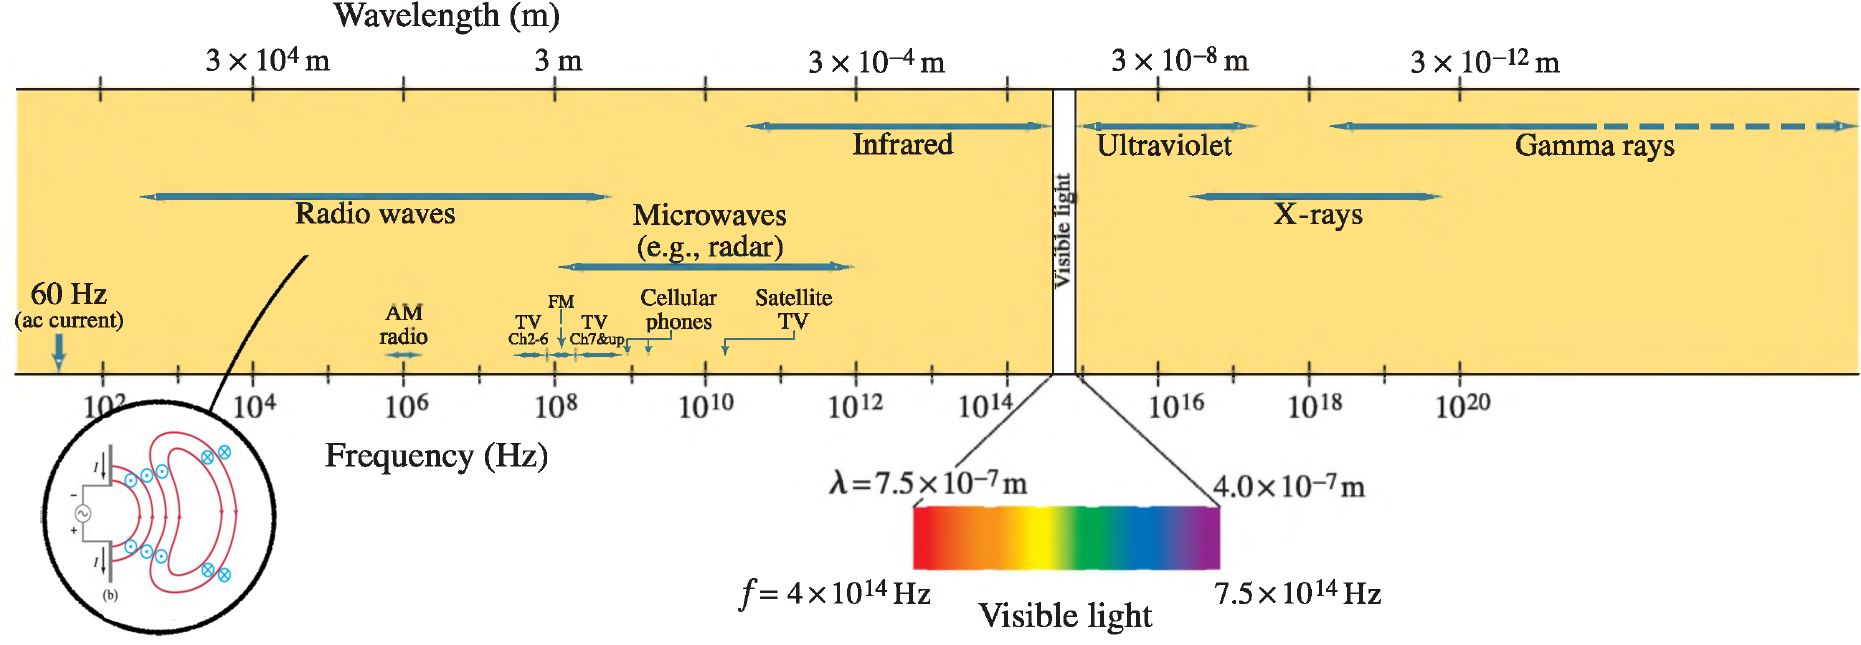
\includegraphics[height=1.5in]{images5/spectrum2.jpg}
\end{center}



  \end{frame}

%%%%%%%%%%%%%%%%%%%%%%%%%%%%%%%%%%%%%%%%%%%%%%%%%%%%%%%%%%%%%%%%%%%


\begin{frame}

\frametitle{Electromagnetic spectrum}

The frequency of light is related with its speed thought the expression,

\begin{equation*}
c=f\lambda
\end{equation*}

  \begin{center}
  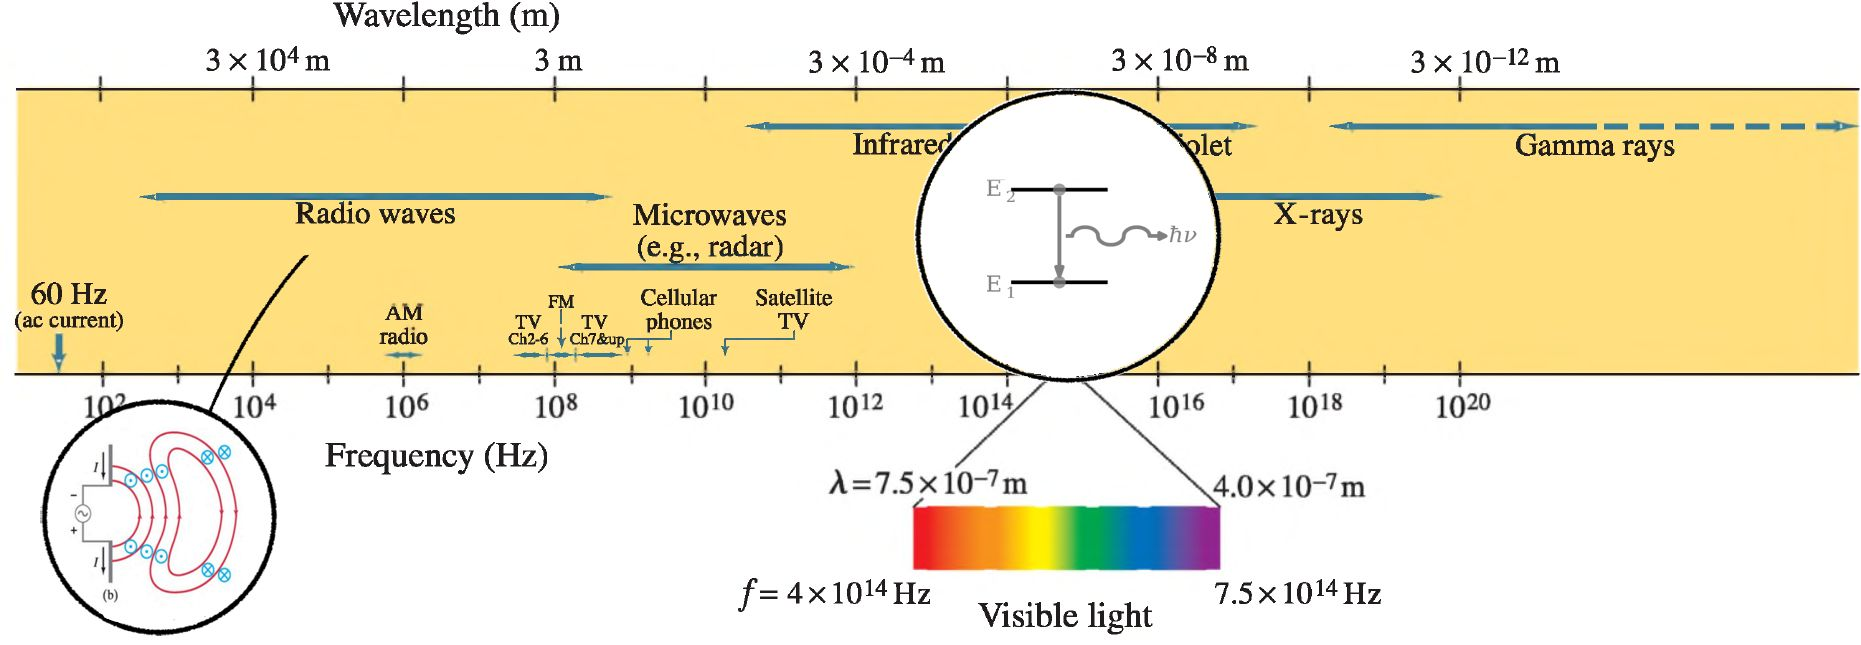
\includegraphics[height=1.5in]{images5/spectrum3.jpg}
\end{center}



  \end{frame}

%%%%%%%%%%%%%%%%%%%%%%%%%%%%%%%%%%%%%%%%%%%%%%%%%%%%%%%%%%%%%%%%%%%


\begin{frame}

\frametitle{Electromagnetic spectrum}

The frequency of light is related with its speed thought the expression,

\begin{equation*}
c=f\lambda
\end{equation*}

  \begin{center}
  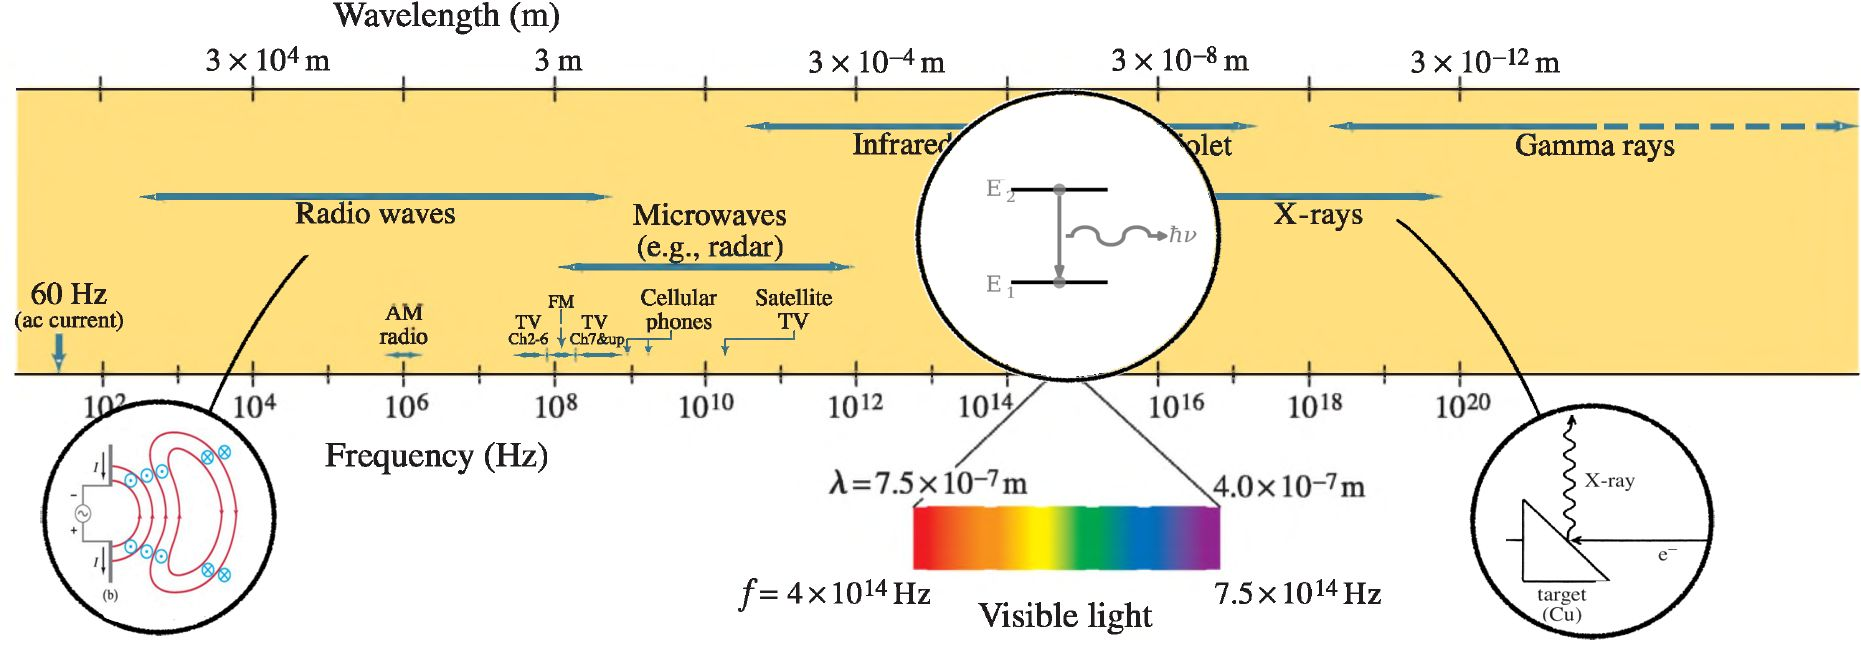
\includegraphics[height=1.5in]{images5/spectrum4.jpg}
\end{center}



  \end{frame}

%%%%%%%%%%%%%%%%%%%%%%%%%%%%%%%%%%%%%%%%%%%%%%%%%%%%%%%%%%%%%%%%%%%


\begin{frame}

\frametitle{Electromagnetic spectrum}

The frequency of light is related with its speed thought the expression,

\begin{equation*}
c=f\lambda
\end{equation*}

  \begin{center}
  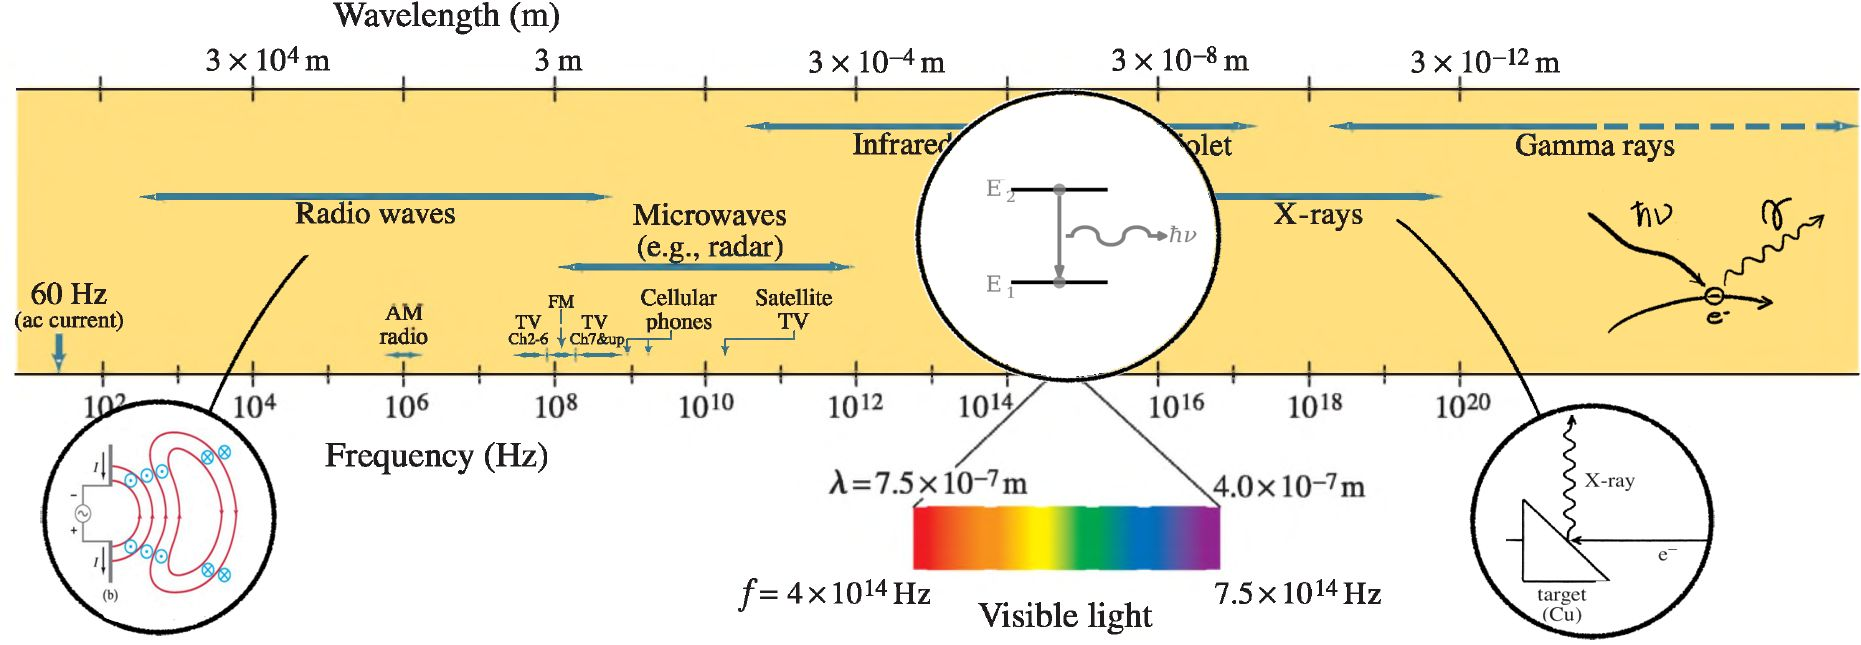
\includegraphics[height=1.5in]{images5/spectrum5.jpg}
\end{center}



  \end{frame}







%%%%%%%%%%%%%%%%%%%%%%%%%%%%%%%%%%%%%%%%%%%%%%%%%%%%%%%%%%%%%%%%%%%


\begin{frame}

\frametitle{Huygens' principle}

\textit{Every point on a wave front can be considered as a source o f tiny
wavelets that spread out in the forward direction at the speed o f the wave itself
The new wave front is the envelope o f all the wavelets— that is, the tangent to all
o f them.}

  \begin{center}
  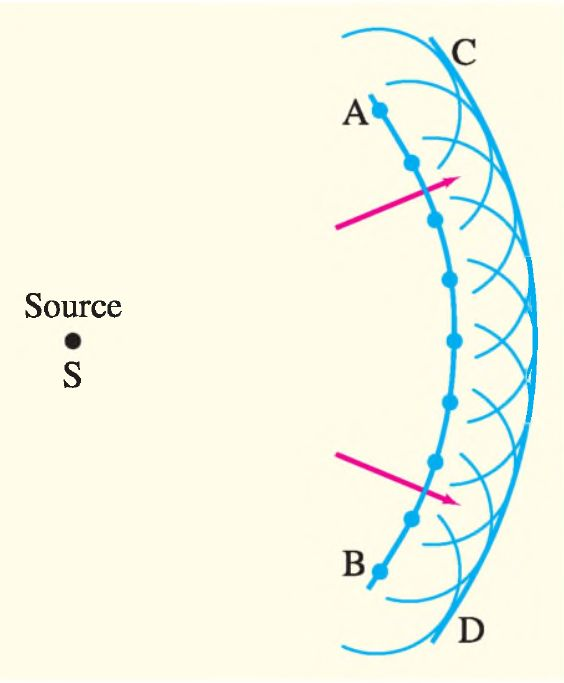
\includegraphics[height=1.3in]{images5/Huygen.jpg}
\end{center}



  \end{frame}




%%%%%%%%%%%%%%%%%%%%%%%%%%%%%%%%%%%%%%%%%%%%%%%%%%%%%%%%%%%%%%%%%%%


\begin{frame}

\frametitle{Diffraction}





   \begin{columns}[c]
   \column{2.8in}  % slides are 3in high by 5in wide

  What happens when waves impinge on an obstacle?
\pause


 $\rightarrow$ waves bend in behind an obstacle
\pause
\vspace{3mm}

 $\rightarrow$The bending into the "shadow region" is known as diffraction
\pause

\vspace{3mm}

 $\rightarrow$ If the opening is much larger then than the wavelength, diffraction goes unnoticed. 
\pause



   \column{1.4in}

  \begin{center}
  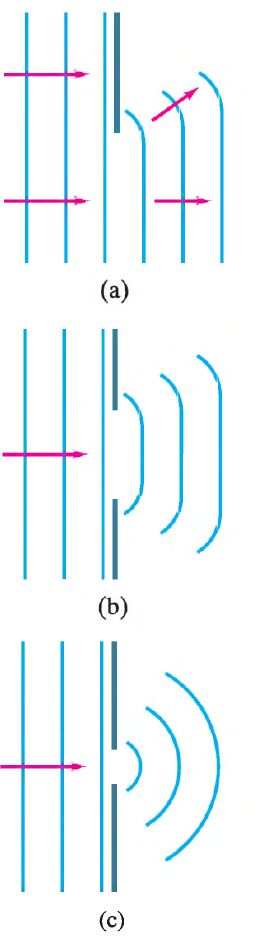
\includegraphics[height=2.3in]{images5/diffraction.jpg}
\end{center}

   \end{columns}




  \end{frame}




%%%%%%%%%%%%%%%%%%%%%%%%%%%%%%%%%%%%%%%%%%%%%%%%%%%%%%%%%%%%%%%%%%%


\begin{frame}

\frametitle{Refraction}

What happens when a waves front changes the medium?
\pause

  \begin{center}
  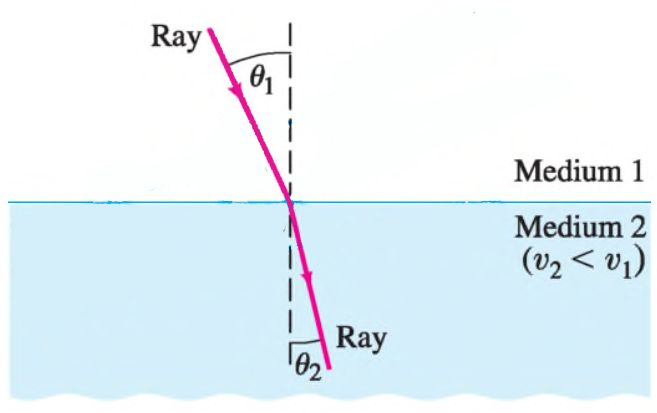
\includegraphics[height=1.8in]{images5/Refraction0.jpg}
\end{center}






  \end{frame}





%%%%%%%%%%%%%%%%%%%%%%%%%%%%%%%%%%%%%%%%%%%%%%%%%%%%%%%%%%%%%%%%%%%


\begin{frame}

\frametitle{Refraction}

We are going to use the Huygens' principle to explain this...
\pause





   \begin{columns}[c]
   \column{2in}  % slides are 3in high by 5in wide

    \begin{center}
  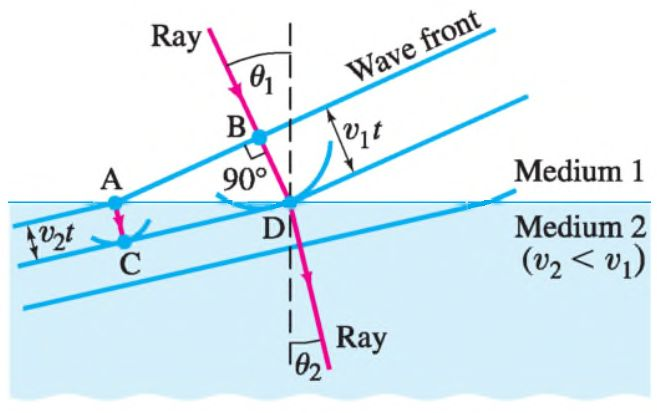
\includegraphics[height=1.5in]{images5/Refraction.jpg}
\end{center}


   \column{2in}

\pause

\begin{equation*}
sin\theta_1=\frac{v_1 t}{AD},\ \ sin\theta_2=\frac{v_2 t }{AD}
\end{equation*}

\pause


\begin{equation*}
\rightarrow \frac{sin\theta_1}{sin\theta_2}=\frac{v_1}{v_2}
\end{equation*}




   \end{columns}


  \end{frame}




%%%%%%%%%%%%%%%%%%%%%%%%%%%%%%%%%%%%%%%%%%%%%%%%%%%%%%%%%%%%%%%%%%%


\begin{frame}

\frametitle{Refraction}



The frequency does not change, but the wavelength does,

\pause

\begin{equation*}
 \frac{\lambda_2}{\lambda_1}=\frac{v_2}{v_1}=\frac{n_1}{n_2}
\end{equation*}
\pause

where,

\begin{equation}
n=\frac{c}{v}
\end{equation}
\pause
\vspace{3mm}

is the \textbf{refraction index}.


  \end{frame}


%%%%%%%%%%%%%%%%%%%%%%%%%%%%%%%%%%%%%%%%%%%%%%%%%%%%%%%%%%%%%%%%%%%


\begin{frame}

\frametitle{Refraction}


Why the velocity change?
\pause

\begin{equation}
v=\frac{1}{\sqrt{\epsilon \mu}}
\end{equation}


$\mu\rightarrow$ The resistance of a material to be penetrated by a magnetic field.

\pause
\vspace{3mm}

$\epsilon\rightarrow$ The resistance of a material to be penetrated by an electric field.



  \end{frame}


%%%%%%%%%%%%%%%%%%%%%%%%%%%%%%%%%%%%%%%%%%%%%%%%%%%%%%%%%%%%%%%%%%%


\begin{frame}

\frametitle{Refraction}


Why the velocity change?
\pause

\begin{equation}
v=\frac{1}{\sqrt{\epsilon \mu}}
\end{equation}


$\mu\rightarrow$ The resistance of a material to be penetrated by a magnetic field.

\pause
\vspace{3mm}

$\epsilon\rightarrow$ The resistance of a material to be penetrated by an electric field.



  \end{frame}





%%%%%%%%%%%%%%%%%%%%%%%%%%%%%%%%%%%%%%%%%%%%%%%%%%%%%%%%%%%%%%%%%%%


\begin{frame}

\frametitle{Refraction}


Example: Mirages

\vspace{3mm}

  \begin{center}
  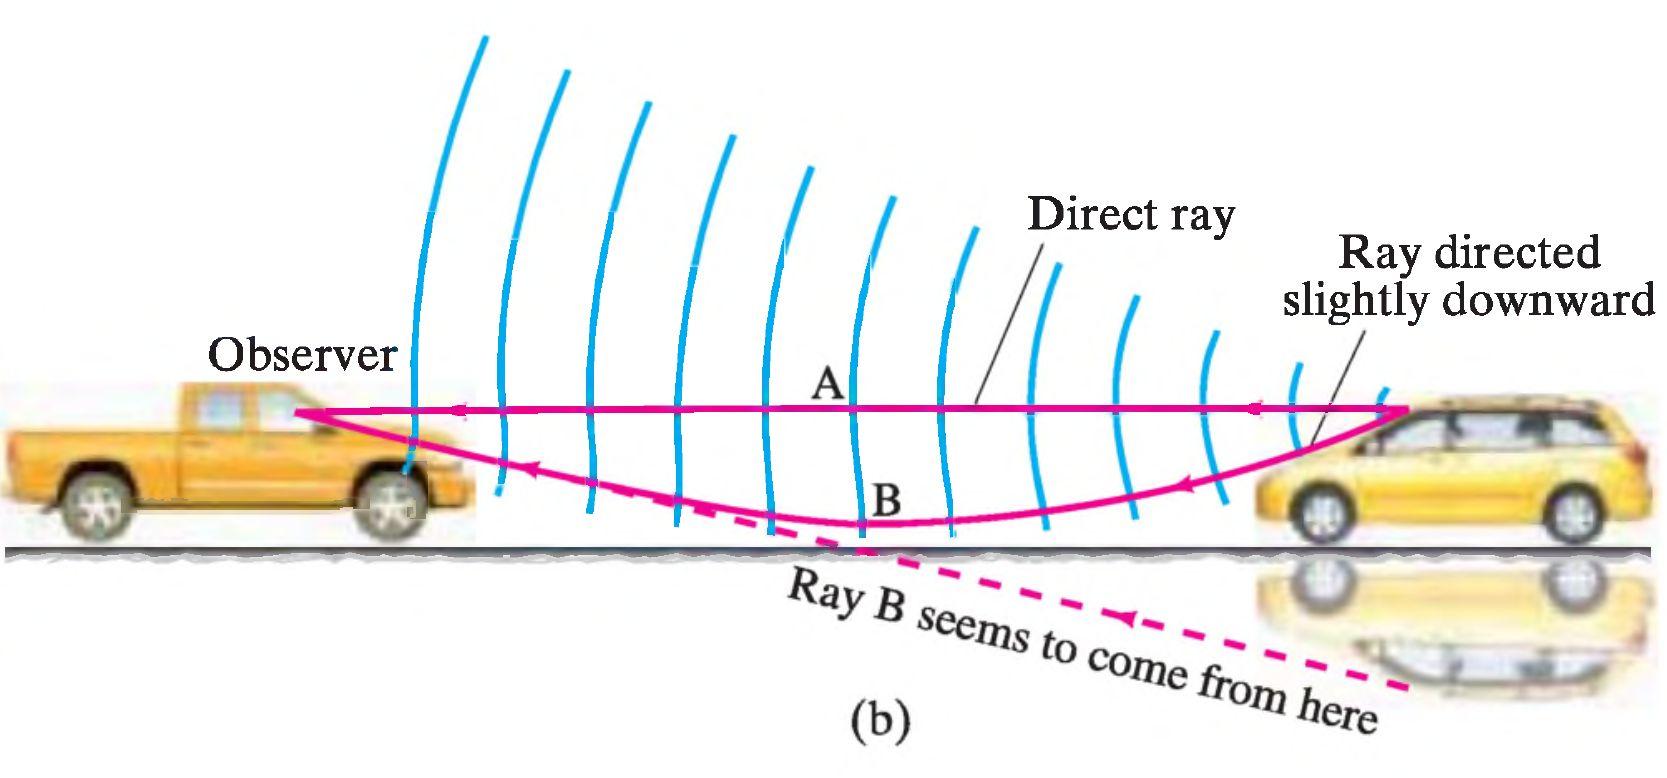
\includegraphics[height=1.7in]{images5/mirages.jpg}
\end{center}


  \end{frame}



%%%%%%%%%%%%%%%%%%%%%%%%%%%%%%%%%%%%%%%%%%%%%%%%%%%%%%%%%%%%%%%%%%%


\begin{frame}

\frametitle{Interference: Youn's double-slit Experiment}



\vspace{3mm}

  \begin{center}
  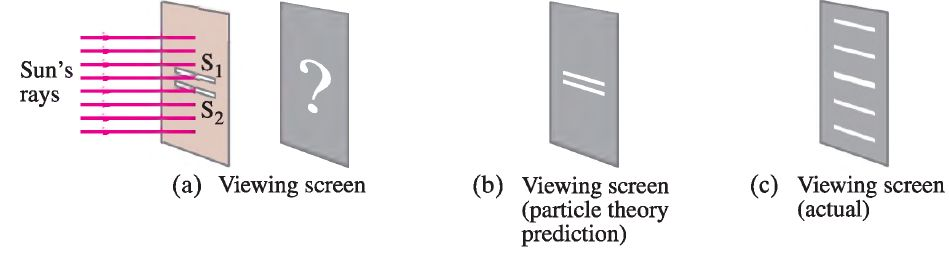
\includegraphics[height=1.2in]{images5/doubleslit.jpg}
\end{center}

\vspace{3mm}

If light consists of tiny particles, we might expect to see two bright lines on a screen placed behind
the slits as in (b). But instead a series of bright lines are seen, as in (c). Young was
able to explain this result as a wave-interference phenomenon.
  \end{frame}











%%%%%%%%%%%%%%%%%%%%%%%%%%%%%%%%%%%%%%%%%%%%%%%%%%%%%%%%%%%%%%%%%%%



%%%%%%%%%%%%%%%%%%%%%%%%%%%%%%%%%%%%%%%%%%%%%%%%%%%%%%%%%%%%%%%%%%%


%\begin{frame}

%\frametitle{Coerence}



%\begin{itemize}
%\item Coherent sources $\rightarrow$ the waves have the same wavelength and frequency, 
%and bear the same phase relationship to each other at all times. 
%\pause 

%\item Incoherent sources $\rightarrow$ waves have phases that bear no fixed relationship to each other 
%over time
%\end{itemize}

%\pause

 %An interference pattern is observed
%only when the sources are coherent. If two tiny lightbulbs replaced the two slits, an
%interference pattern would not be seen. The light emitted by one lightbulb would
%have a random phase with respect to the second bulb, and the screen would be
%more or less uniformly illuminated. 

%  \end{frame}



  
  








%%%%%%%%%%%%%%%%%%%%%%%%%%%%%%%%%%%%%%%%%%%%%%%%%%%%%%%%%%%%%%%%%%%


\begin{frame}

\frametitle{Interference in Thin Films}

  \begin{center}
  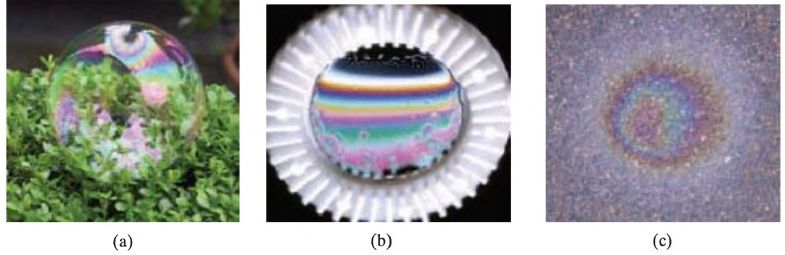
\includegraphics[height=1.5in]{images5/soap.jpg}
\end{center}


  \end{frame}







%%%%%%%%%%%%%%%%%%%%%%%%%%%%%%%%%%%%%%%%%%%%%%%%%%%%%%%%%%%%%%%%%%%


% \begin{frame}

% \frametitle{Colors in a Thin Soap Film}




%   \begin{columns}[c]
%    \column{2in}  % slides are 3in high by 5in wide
  
  
%      \begin{center}
%   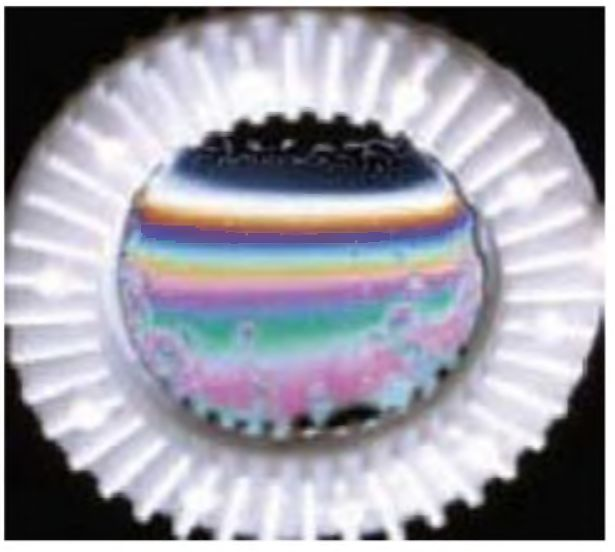
\includegraphics[height=1.7in]{images5/soap3.jpg}
% \end{center}


%    \column{2in}

  
%   \begin{itemize}
%   \item The thin film  stood vertically.
%   \pause
%  \item  Gravity has pulled much of the soapy water toward the bottom.
 
%  \pause
% \item The top section is so thin $\rightarrow$ light reflected from the front and
% back surfaces have almost no path difference.

% \pause

% \item 180$^{\circ}$ $\rightarrow$  two reflected waves are  out of phase for all wavelengths.

 
  
%   \end{itemize}
  


%    \end{columns}




%   \end{frame}



%%%%%%%%%%%%%%%%%%%%%%%%%%%%%%%%%%%%%%%%%%%%%%%%%%%%%%%%%%%%%%%%%%%


\begin{frame}

\frametitle{Colors in a Thin Soap Film}


  
     \begin{center}
  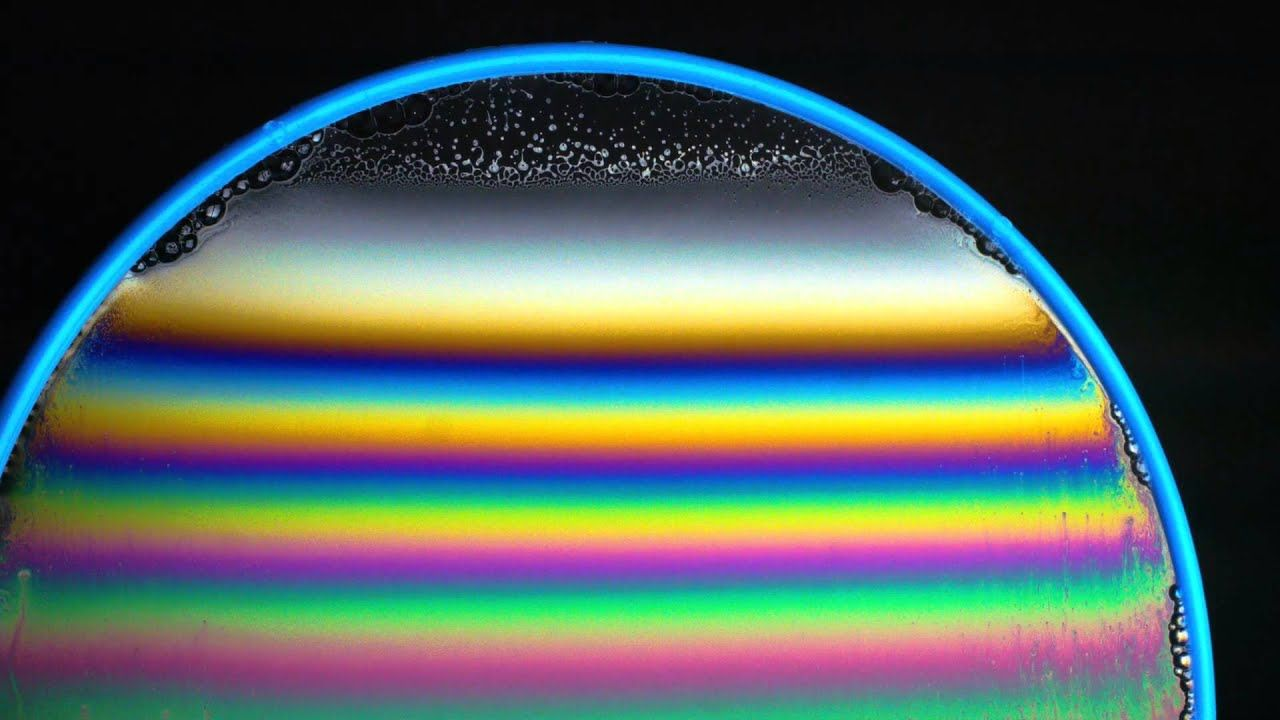
\includegraphics[height=2.0in]{images5/soap4.jpg}
\end{center}



  \end{frame}

%%%%%%%%%%%%%%%%%%%%%%%%%%%%%%%%%%%%%%%%%%%%%%%%%%%%%%%%%%%%%%%%%%%























%%%%%%%%%%%%%%%%%%%%%%%%%%%%%%%%%%%%%%%%%%%%%%%%%%%%%%%%%%%%%%%
 \end{document}
%%%%%%%%%%%%%%%%%%%%%%%%%%%%%%%%%%%%%%%%%%%%%%%%%%%%%%%%%%%%%%%